\documentclass[11pt]{beamer}
\usepackage{listings} % Include the listings-package
\usepackage[T1]{fontenc}
\usepackage[utf8]{inputenc}
\usepackage[english]{babel}
\usepackage{amsmath}
\usepackage{amssymb, amsfonts, latexsym, cancel}
\usepackage{float}
\usepackage{graphicx}
\usepackage{epstopdf}
\usepackage{subfigure}
\usepackage{hyperref}
%\usepackage{authblk}
\usepackage{blindtext}
\usepackage{booktabs} % Allows the use of \toprule, 
\usepackage{filecontents}
\usepackage{courier} %% Sets font for listing as Courier.
\usepackage{listings}
%\usepackage{listings, xcolor}
\lstset{
tabsize = 2, %% set tab space width
showstringspaces = false, %% prevent space marking in strings, string is defined as the text that is generally printed directly to the console
numbers = left, %% display line numbers on the left
commentstyle = \color{green}, %% set comment color
keywordstyle = \color{blue}, %% set keyword color
stringstyle = \color{red}, %% set string color
rulecolor = \color{black}, %% set frame color to avoid being affected by text color
basicstyle = \small \ttfamily , %% set listing font and size
breaklines = true, %% enable line breaking
numberstyle = \tiny,
}
\usepackage{caption}
\DeclareCaptionFont{white}{\color{white}}
\DeclareCaptionFormat{listing}{\colorbox{gray}{\parbox{\textwidth}{#1#2#3}}}
\captionsetup[lstlisting]{format=listing,labelfont=white,textfont=white}
\definecolor{urlColor}{rgb}{0.06, 0.3, 0.57}
\definecolor{linkColor}{rgb}{0.57, 0.0, 0.04}
\definecolor{fileColor}{rgb}{0.0, 0.26, 0.26}
\hypersetup{
    colorlinks=true,
    linkcolor=linkColor,
    filecolor=fileColor,      
    urlcolor=urlColor,
}
\urlstyle{same}
\setbeamercovered{transparent}
%\usetheme{Boadilla}
\usetheme{CambridgeUS}
%\usetheme{Berkeley}
%\usetheme{Warsaw}
%\usetheme{Madrid}

\title[Smith y Mosier]{\bf\Huge Smith y Mosier  }


\author[]
{
    Alvan Ventura Edsel\inst{1}\\
	Chuctaya Ruiz Diego \inst{2}\\
	Santos Cruz Esteba \inst{3}\\
	Ramos Ticona Gilbert\inst{4}
}
\institute[UNSA]
{
\inst{1}% 
System Engineering School\\
}
\date[2020-09-15]{\scriptsize{2020-09-15}}
%\logo{
\includegraphics[width=3.0cm]{img/logo_unsa.jpg}}
\titlegraphic{
\includegraphics[width=1.0cm]{logo_unsa.jpg}}
\begin{document}

\begin{frame}
\titlepage
\end{frame}

\begin{frame}
\frametitle{Content}
\tableofcontents
\end{frame}

\section{OBJETIVOS Smith y Mosier}
\begin{frame}
\frametitle{OBJETIVOS Smith y Mosier}
\begin{itemize}
 \item Consistencia. En terminología así como en formato\\
 \item Asimilación eficiente de la información por parte del usuario\\
 \item Minimizar la carga de la memoria del usuario\\
 \item Compatibilidad entre el despliegue y la entrada\\
 \item Flexibilidad para el usuario, en las formas de despliegue


\begin{figure}[t]
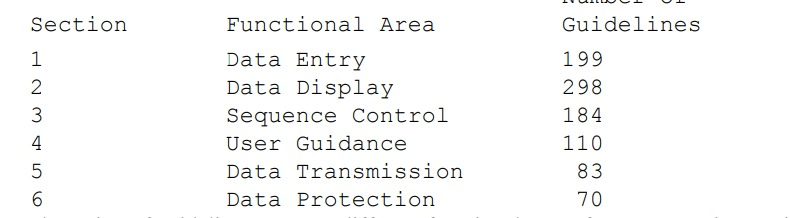
\includegraphics[width=8cm, height=4cm]{SmithMosier.jpg}
\centering
\end{figure}
\end{itemize}
\end{frame}

\section{BUSCAMOS Y USAMOS ESTRUCTURA VISUAL}
%References frame
\begin{frame}
\frametitle{BUSCAMOS Y USAMOS ESTRUCTURA VISUAL}
\begin{itemize}
\item La presentación estructurada se puede escanear y comprender mucho más rápidamente que la presentación en prosa.
\item Cuanto más estructurada y concisa sea la presentación de la información, más rápida y fácilmente la gente podrá escanearla y comprenderla.

\begin{figure}[t]
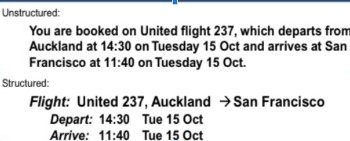
\includegraphics[width=8cm, height=4cm]{Estructura.jpg}
\centering
\end{figure}
\end{itemize}
\end{frame}



%References frame
\begin{frame}
\frametitle{LA LECTURA ES ANTINATURAL}
\begin{itemize}
\item La redacción o presentación descuidadas del texto puede reducir la lectura automática y sin contexto de los lectores expertos a una lectura consciente basada en el contexto, lo que sobrecarga la memoria de trabajo y, por lo tanto, disminuye la velocidad y la comprensión. En lectores no calificados, la presentación deficiente del texto puede bloquear la lectura por completo.

\begin{figure}[t]
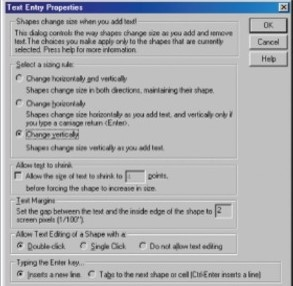
\includegraphics[width=8cm, height=4cm]{data.jpg}
\centering
\end{figure}
\end{itemize}
\end{frame}

%References frame
\begin{frame}
\frametitle{SIGNIFICADO DE LA INTERFAZ DE USUARIO}
\begin{itemize}
\item El diseño del software de interfaz de usuario es fundamental para el rendimiento eficaz del sistema\\
Una interfaz debe ser  fácil de usar (explicarse por sí misma), eficiente y agradable\\
Cuando un sistema falla, el resultado es una operación interrumpida, una pérdida de tiempo, esfuerzo y dinero, y la imposibilidad de lograr los beneficios potenciales del manejo automatizado de la información.


\begin{figure}[t]

\includegraphics[width=8cm, height=4cm]{logo.jpg}
\centering
\end{figure}
\end{itemize}
\end{frame}

\begin{frame}
\frametitle{PRÁCTICA DE DISEÑO}
\begin{itemize}
\item El diseño actual de software de interfaz de usuario es arte más que ciencia\\
Como arte, el diseño de la interfaz de usuario lo practican mejor los expertos, pero no siempre están disponibles\\
Gracias a una práctica en un sistema de información militar reveló que el curso real del desarrollo de software de interfaz de usuario a veces se apartará de la secuencia deseada



\begin{figure}[t]
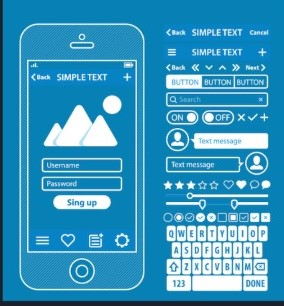
\includegraphics[width=8cm, height=4cm]{table.jpg}
\centering
\end{figure}
\end{itemize}
\end{frame}

\section{References}
%References frame
\begin{frame}
\frametitle{References}
\begin{itemize}
\item Intdrouction - xiii, Jhonson J. (2014). Designing with the Mind in mind. 2nd. edition.
\item Sidney L. Smith and Jane N. Mosier \\
Albert, A. E. (1982). The effect of graphic input devices on performance in a cursor positioning task. 

\item In Proceedings of the Human Factors Society 26th Annual Meeting (pp. 54-58). Santa Monica, CA: Human Factors Society..
\end{itemize}
\end{frame}

\end{document}
